\section{Anhang}
\subsection{\emph{MArC} ReadMe-Datei}\label{sec:readMe}
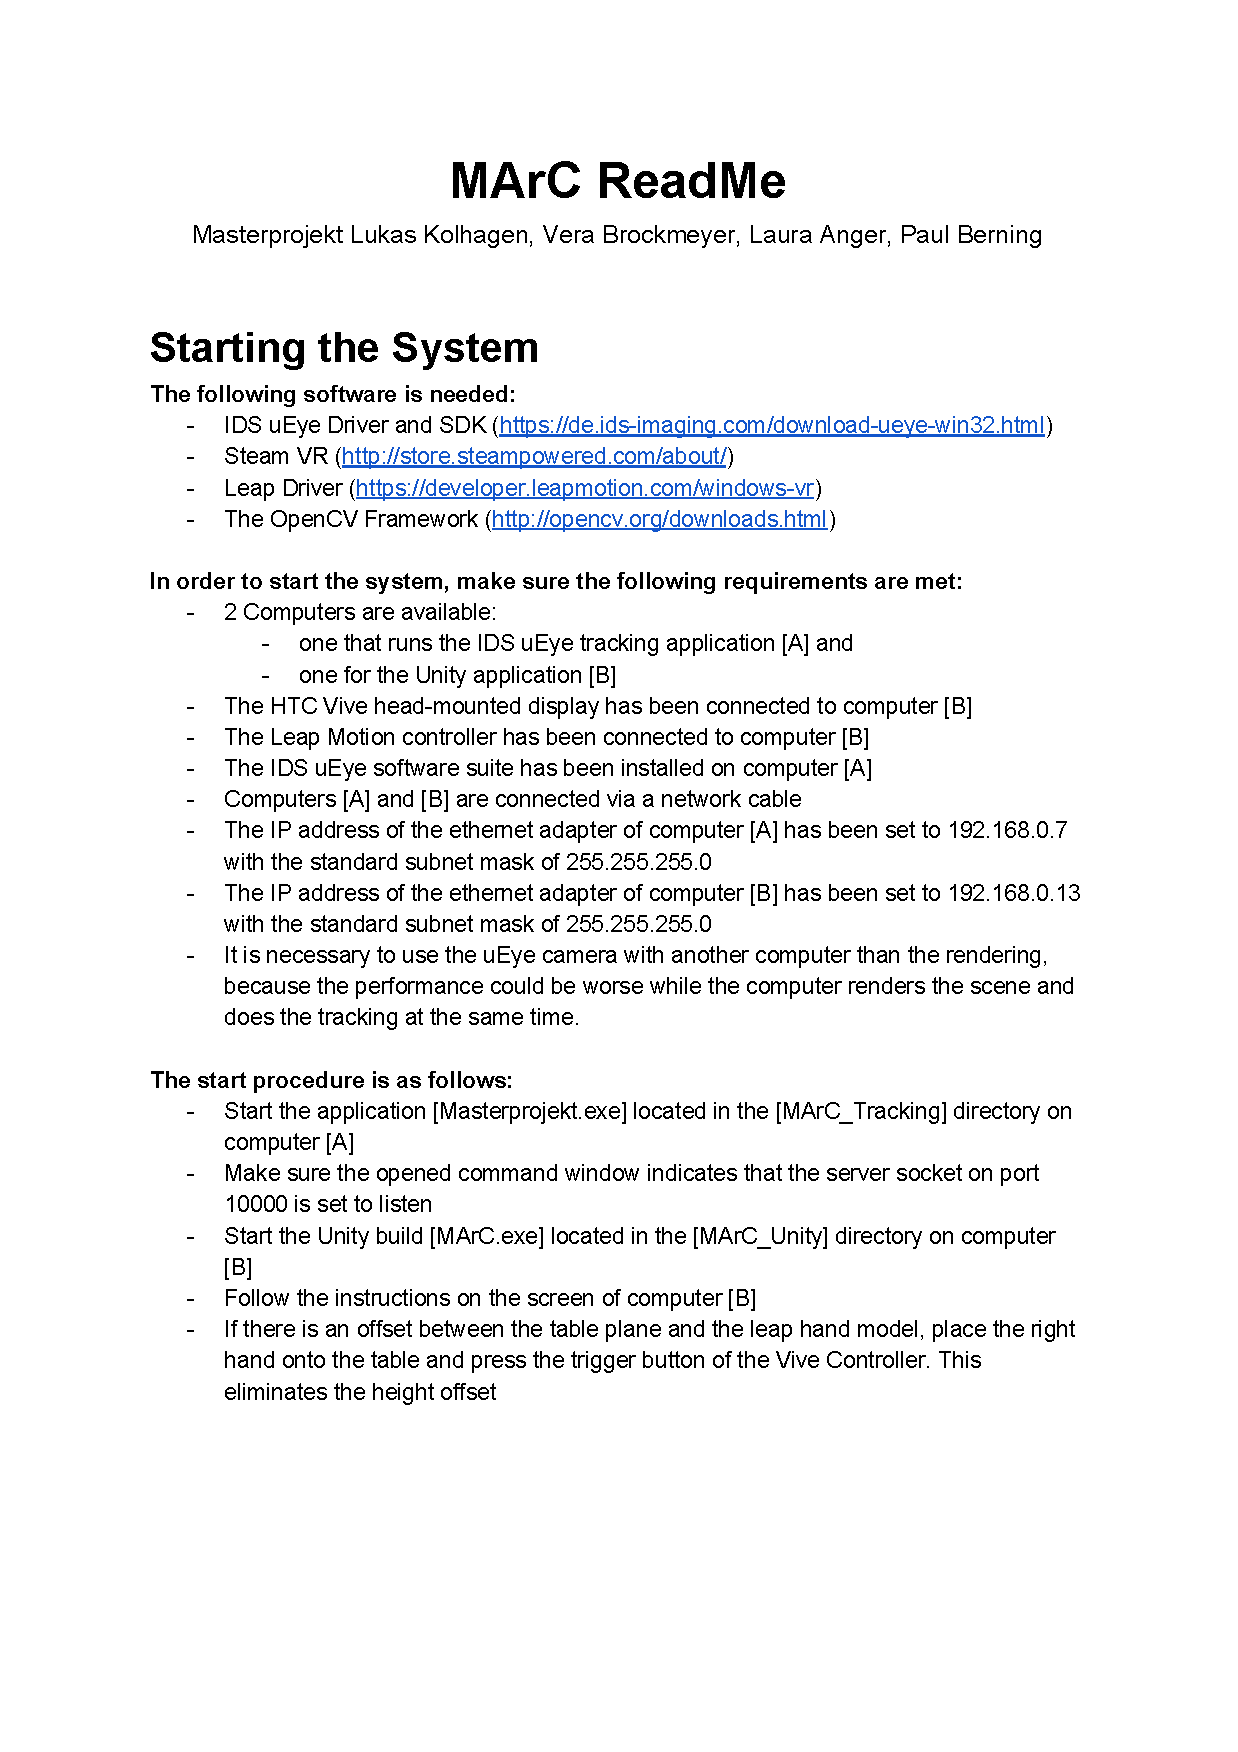
\includepdf[pages=-]{kapitel/anhang/ReadMe.pdf} 

\subsection{Schachbrett zum Ausdrucken}

\begin{figure}[H] 
	\center 
	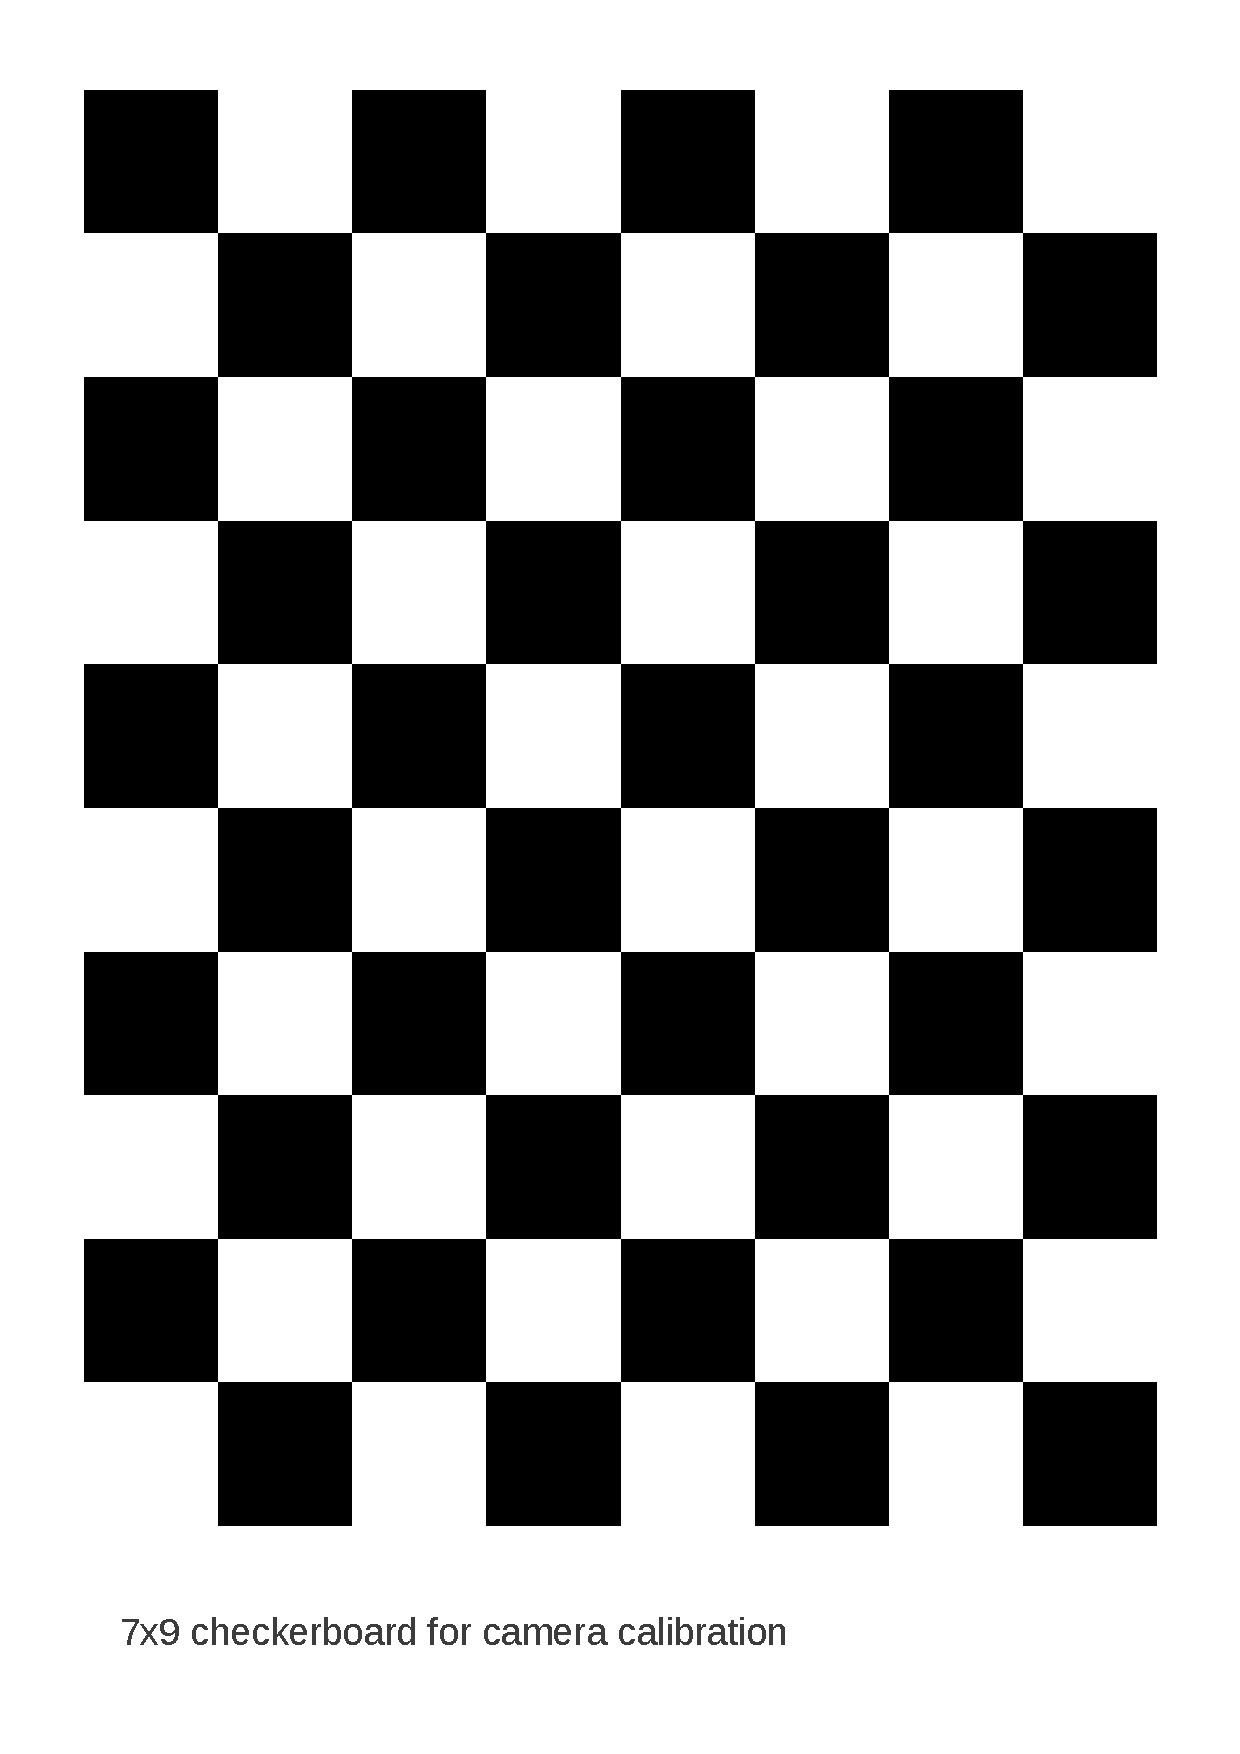
\includegraphics[scale=0.75]{Bilder/camera-calibration-checker-board_9x7.pdf}			
	\caption{Um den Faktor 0.75 skaliertes $7\times9$ Schachbrett.}
	\label{fig:schachbrett}
\end{figure}

Download unter \url{http://www.mrpt.org/downloads/camera-calibration-checker-board_9x7.pdf} (Abgerufen am: 25.03.2017).

\subsection{\texttt{startTCPServer()}-Methode}
\lstinputlisting[title=\lstname, caption={\texttt{startTCPServer()}-Methode in \texttt{TCP.cpp}}, label=lst:startTCPServer, language={C++}, linerange=22-77, firstnumber=22]{Quellcode/TCP.cpp}

\subsection{\texttt{getPointerOfMarkerVec()}-Methode}
\lstinputlisting[title=\lstname, caption={\texttt{getPointerOfMarkerVec()}-Methode in \texttt{TCP.cpp}}, label=lst:getPointerOfMarkerVec, language={C++}, linerange=131-164, firstnumber=131]{Quellcode/TCP.cpp} 

\subsection{\texttt{interpretTCPMarkerData()}-Methode}
\lstinputlisting[title=\lstname, caption={\texttt{interpretTCPMarkerData()}-Methode in \texttt{readInNetWorkData.cs}}, label=lst:interpretData, language={[Sharp]C}, linerange=141-174, firstnumber=141]{Quellcode/readInNetworkData.cs}

\subsection{\texttt{runCalibWithChessboard()}-Methode}
\lstinputlisting[title=\lstname, caption={\texttt{runCalibWithChessboard()}-Methode in \texttt{calibWithChessboard.cpp}}, label=lst:runCalibWithChessboard, language={[Sharp]C}, linerange=146-349, firstnumber=146]{Quellcode/calibWithChessboard.cpp}

\subsection{\texttt{runCalibration()}-Methode}
\lstinputlisting[title=\lstname, caption={\texttt{runCalibration()}-Methode in \texttt{calibWithChessboard.cpp}}, label=lst:runCalibration, language={[Sharp]C}, linerange=71-103, firstnumber=71]{Quellcode/calibWithChessboard.cpp}


